\documentclass[12pt,a4paper,final]{beamer}
\usetheme{PaloAlto}

\usepackage[utf8]{inputenc}
\usepackage[portuguese]{babel}
\usepackage[T1]{fontenc}
\usepackage{graphicx}

\author{Warley Santos}
\title{Informática Básica Aula 1}
\institute{Associação Gesto de Amor}
\date{2018}
\logo{
\includegraphics[scale=0.058]{imagens/logo.jpg}}

\AtBeginSection[]{
    \begin{frame}
        \tableofcontents[currentsection, hideothersubsections]
    \end{frame}
}

\begin{document}
% Page 1
	\begin{frame}
		\titlepage
	\end{frame}
% Page 2
	\begin{frame}
	    \frametitle{Sumario}
		\tableofcontents
	\end{frame}
% Page 3
    \section{O que é informática?}
        \subsection{Concepção}
            \begin{frame}
                \frametitle{O que é Informática?}
                \framesubtitle{Concepção}
                \begin{block}{Origem da palavra:}
                    Em 1956, o cientista da computação alemão \textbf{Karl Steinbuch} publicou o periódico:
                 \end{block}
                 \begin{block}{}
                    \emph{\textbf{Informática:} Processamento Automático de Informação}
                \end{block}
                \begin{block}{}
                     \centering
                     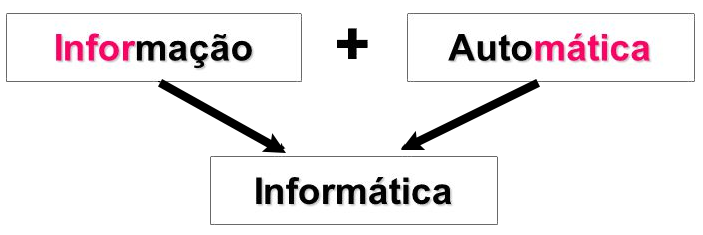
\includegraphics[scale=0.3]{Imagens/informatica.png}
                \end{block}
            \end{frame}
% Page 3
        \subsection{Pirâmide do Conhecimento}
            \begin{frame}
                \frametitle{O que é Informática?}
                \framesubtitle{Pirâmide do Conhecimento}
                    \begin{block}{}
                         \centering
                         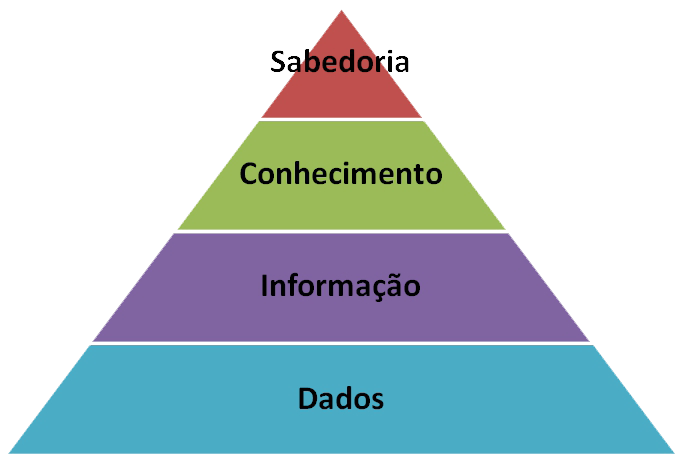
\includegraphics[scale=0.5]{Imagens/piramede.png}
                    \end{block}
	        \end{frame}
% Page 4
    \section{História}
        \subsection{Dígito}
            \begin{frame}
                \frametitle{Um Pouco de história}
                \framesubtitle{Dígito}
                \begin{block}{Nos primórdios:}
                    Primeira maneira que os seres humanos encontraram para expressar quantidade.
                \end{block}
                \begin{block}{}
                    \centering
                    \textcolor{blue}{\large \textbf{Digitus = Dedo, em latim}}
                \end{block}
                \begin{block}{}
                     \centering
                     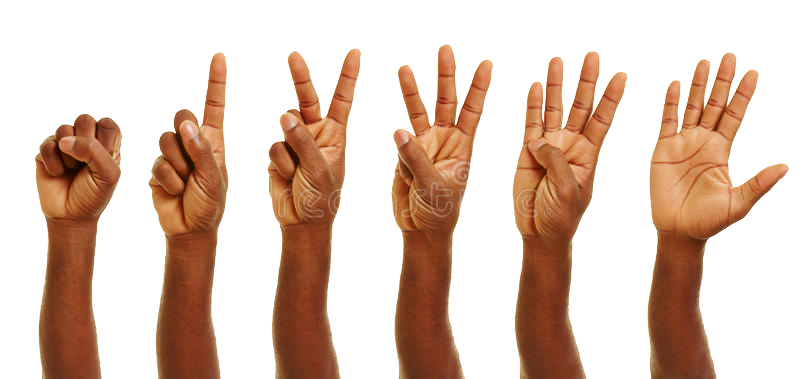
\includegraphics[scale=1]{Imagens/maos.png}
                \end{block}
            \end{frame}
% Page 5
        \subsection{Calculo}
            \begin{frame}
                \frametitle{Um Pouco de história}
                \framesubtitle{Calculo}
                \begin{block}{Nos primórdios:}
                    Empilhamento de pedrinhas para saber a quantidade de ovelhas no rebanho.
                \end{block}
                \begin{block}{}
                    \centering
                    \textcolor{blue}{\large \textbf{Calculus = Pedra, em latim}}
                \end{block}
                \begin{block}{}
                     \centering
                     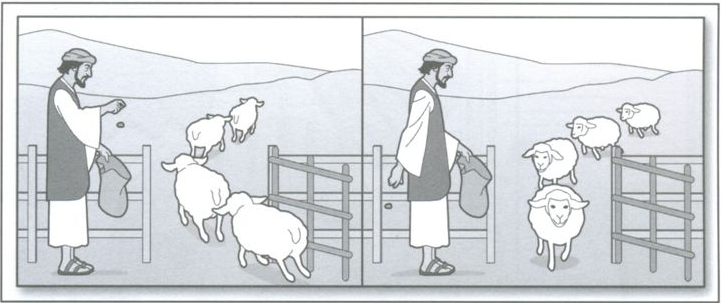
\includegraphics[scale=0.4]{Imagens/ovelhas.png}
                \end{block}
            \end{frame}
% Page 6
        \subsection{Ábaco}
            \begin{frame}
                \frametitle{Um Pouco de história}
                \framesubtitle{Ábaco}
                \begin{block}{Nos primórdios:}
                   Foi um dos primeiros instrumentos desenvolvidos para auxiliar os humanos na realização de cálculos. Existem evidências deles na Babilônia no ano 300 A.C.
                \end{block}
                \begin{block}{}
                     \centering
                     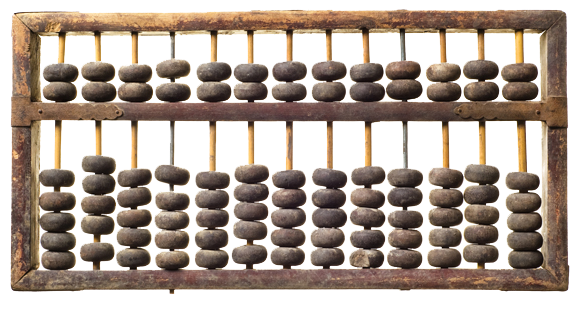
\includegraphics[scale=1.2]{Imagens/abaco.png}
                \end{block}
            \end{frame}
% Page 7
        \subsection{Outras Máquinas}
            \begin{frame}
                \frametitle{Um Pouco de história}
                \framesubtitle{Outras Máquinas}
                \begin{minipage}{.6\linewidth}
                    Napier inventou o que ficou conhecido por \textbf{"Ossos de Napier}", que auxiliavam na realização de multiplicações, baseando-se na teoria de logaritmos.    
                \end{minipage}
                \begin{minipage}{.3\linewidth}
                    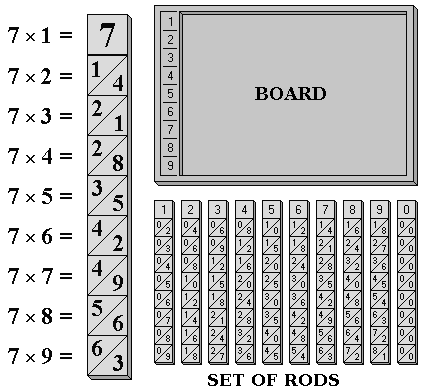
\includegraphics[scale=0.2]{Imagens/napier.jpg}
                \end{minipage}
                \begin{minipage}{.3\linewidth}
                    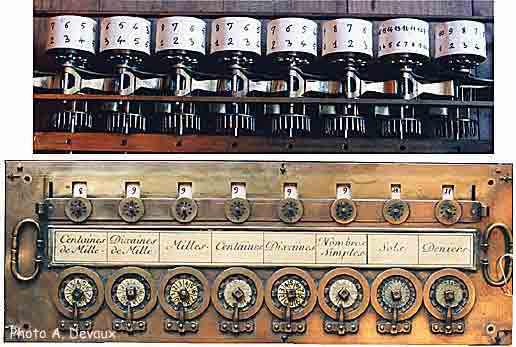
\includegraphics[scale=0.15]{Imagens/pascaline.jpg}
                \end{minipage}           
                \begin{minipage}{.6\linewidth}
Em 1642, o francês \textbf{Blaise Pascal}, aos 19 anos de idade auxiliava o pai na realização de cálculos. Mas, o trabalho era muito entediante, o que o levou a elaborar um dispositivo para realização de somas e subtração.  
                \end{minipage}
            \end{frame}
% Page 8
        \subsection{Máquina Analítica}
            \begin{frame}
                \frametitle{Um Pouco de história}
                \framesubtitle{Máquina Analítica e os cartões perfurados}
                \begin{block}{Em 1837:}
                \begin{itemize}
                    \item \textbf{Charles Babbage} anunciou um projeto para construção da \textbf{Máquina Analítica}. Influenciado por um tear, Babbage propôs uma máquina de propósito genérico, utilizando uma programação através de cartões perfurados.
                    \item Ele idealizou o que hoje chamamos de \textbf{unidade de armazenamento} e \textbf{unidade de processamento de dados}.
                \end{itemize}
                \end{block}
            \end{frame}
% Page 9
            \begin{frame}
                \frametitle{Um Pouco de história}
                \framesubtitle{Máquina Analítica e os cartões perfurados}
                \begin{block}{}
                     \centering
                     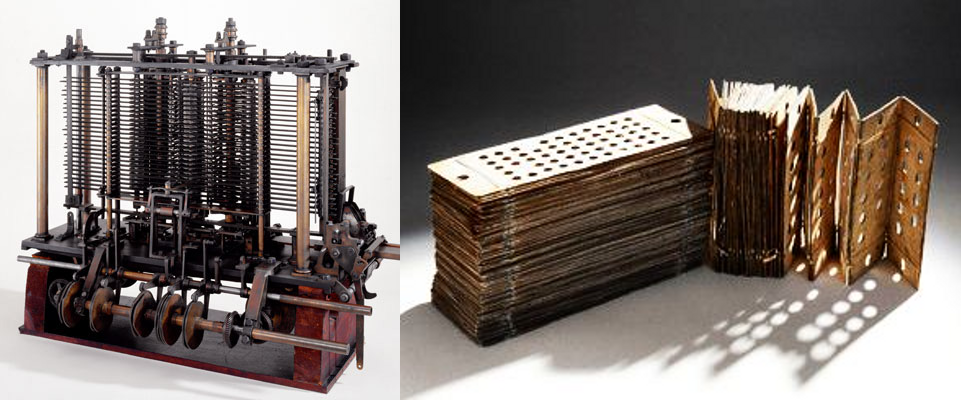
\includegraphics[scale=.34]{Imagens/analitica.png}
                \end{block}
            \end{frame}
% Page 10
            \begin{frame}
                \frametitle{Um Pouco de história}
                \framesubtitle{Máquina Analítica e os cartões perfurados}         
                \begin{block}{Primeira Programadora}
                    \begin{minipage}{.5\linewidth}
A condessa de Lovelace, Ada Byron, se interessou pela máquina analítica de Babbage e passou a escrever programas que a máquina poderia ser capaz de executar.
                    \end{minipage}
                    \begin{minipage}{.4\linewidth}
                        \centering
                        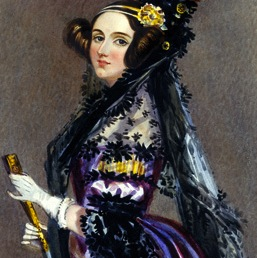
\includegraphics[scale=.4]{Imagens/ada.jpg}
                    \end{minipage}
                \end{block}
            \end{frame}
%%%%%%%%%%%%%%%%%%%%%%%%%%%%%%%%%
    \section{Noções Básicas}
        \subsection{Hardware x Software}
            \begin{frame}
                \centering
                \frametitle{Noções Básicas}
                \framesubtitle{Hardware x Software}
                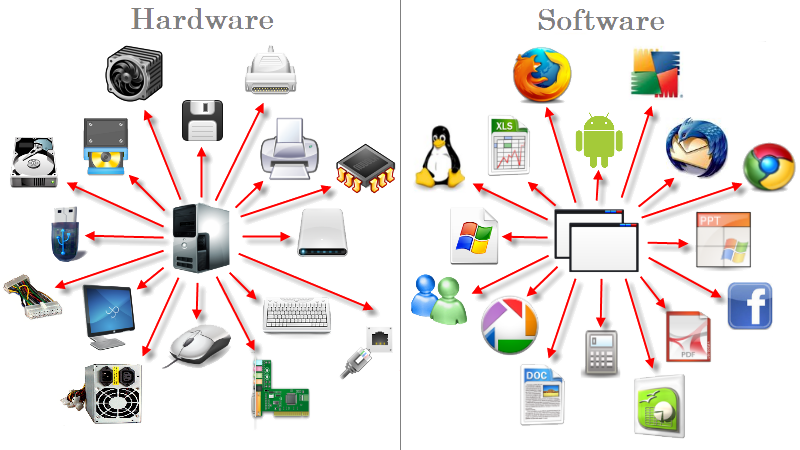
\includegraphics[scale=.3]{Imagens/hardSoft.png}
                \begin{itemize}             
                    \item O conceito de \textbf{hardware} engloba todos os dispositivos físicos e equipamentos utilizados no processo de informações.\item O \textbf{software} é a parte lógica, o conjunto de instruções e dados processados pelos circuitos eletrônicos do hardware.
                \end{itemize}
            \end{frame}
%%%%%%%%%%%%%%%%%%%%%%%%%%%%%%%%%%%%%%%%%%%%%%%%%%%%%%%%%%%%%%%%%%%%%%%%%%%%%%%%%%%%%%%%%%%%%%%%%%%%%
            \subsection{Sistema Computacional}
            \begin{frame}
                \frametitle{Noções Básicas}
                \framesubtitle{Sistema Computacional}
                \begin{block}{Pilha do Sistema Computacional}
                    \centering
                    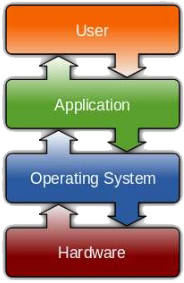
\includegraphics[scale=.5]{Imagens/sistemaComputacional.png}                
                \end{block}
            \end{frame}
            
        \end{document}